\graphicspath{ {./content/exp/figure/} }

\section{Experiments and results}\label{sec:4}

\subsection{Experimental setup}


	%\graphicspath{ {./Figure/Figure6/} }
\begin{figure}
  \centering
  \hspace*{\fill}
  %\subfigure[]{\label{subfig:4a}\includegraphics[width=0.3\linewidth]{fig4a.png}} \hfill
  %\subfigure[]{\label{subfig:4b}\includegraphics[width=0.3\linewidth]{fig4b.png}} 
  %\hspace*{\fill} \\ \hspace*{\fill}
  %\subfigure[]{\label{subfig:4c}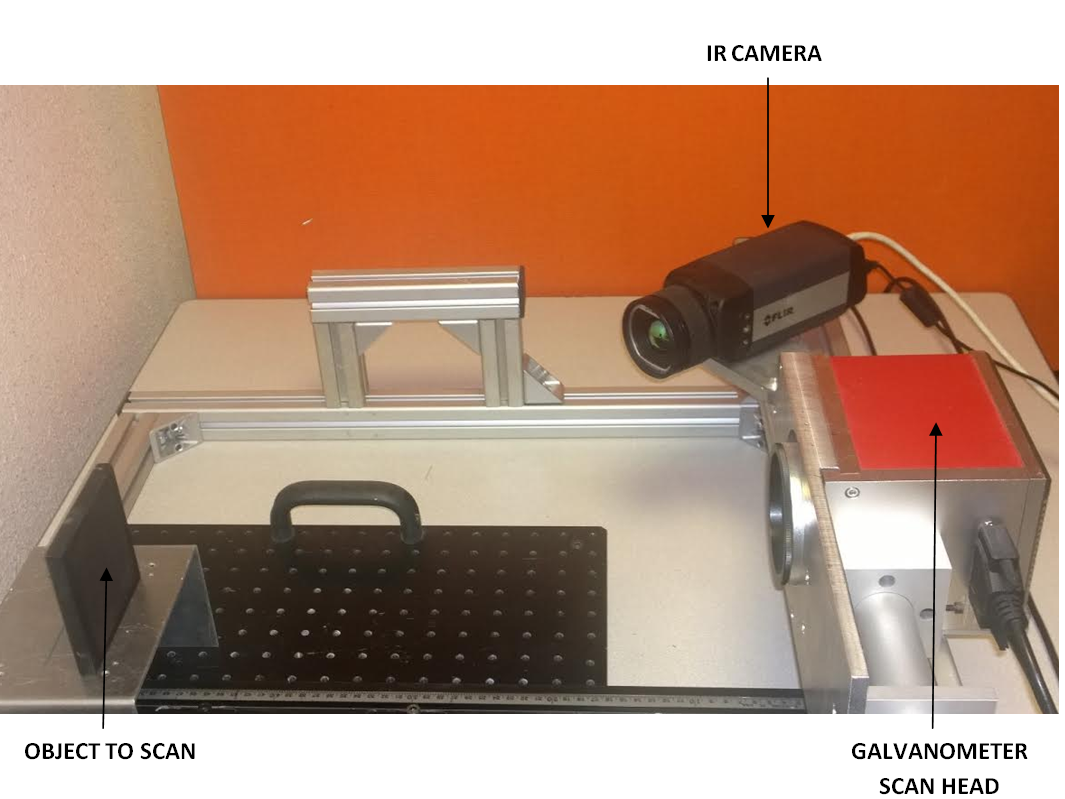
\includegraphics[width=0.3\linewidth]{fig4c.png}}
	{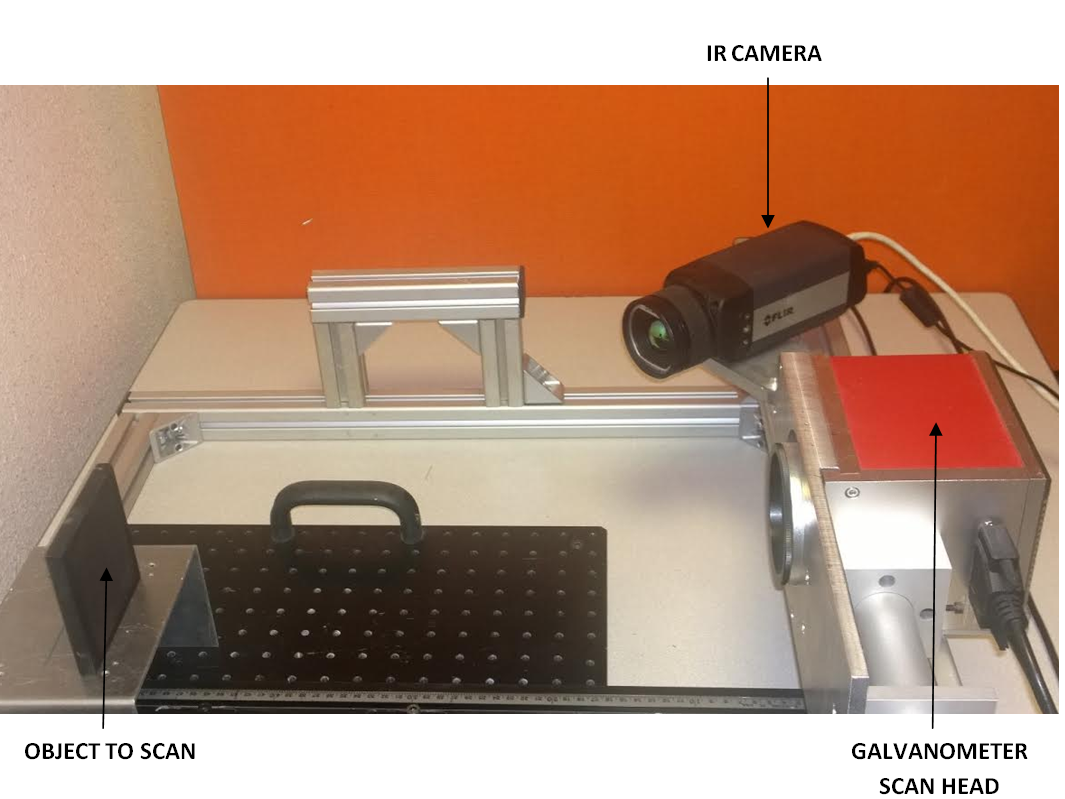
\includegraphics[width=0.7\linewidth]{fig4c.png}}
  \hspace*{\fill}
	
	\caption{Scanner prototype.}
  \label{fig:4}
\end{figure}
  

%\begin{figure}
  %\centering
  %\hspace*{\fill}
  %%\subfigure[]{\label{subfig:4a}\includegraphics[width=0.3\linewidth]{fig4a.png}} \hfill
  %%\subfigure[]{\label{subfig:4b}\includegraphics[width=0.3\linewidth]{fig4b.png}} 
  %%\hspace*{\fill} \\ \hspace*{\fill}
  %%\subfigure[]{\label{subfig:4c}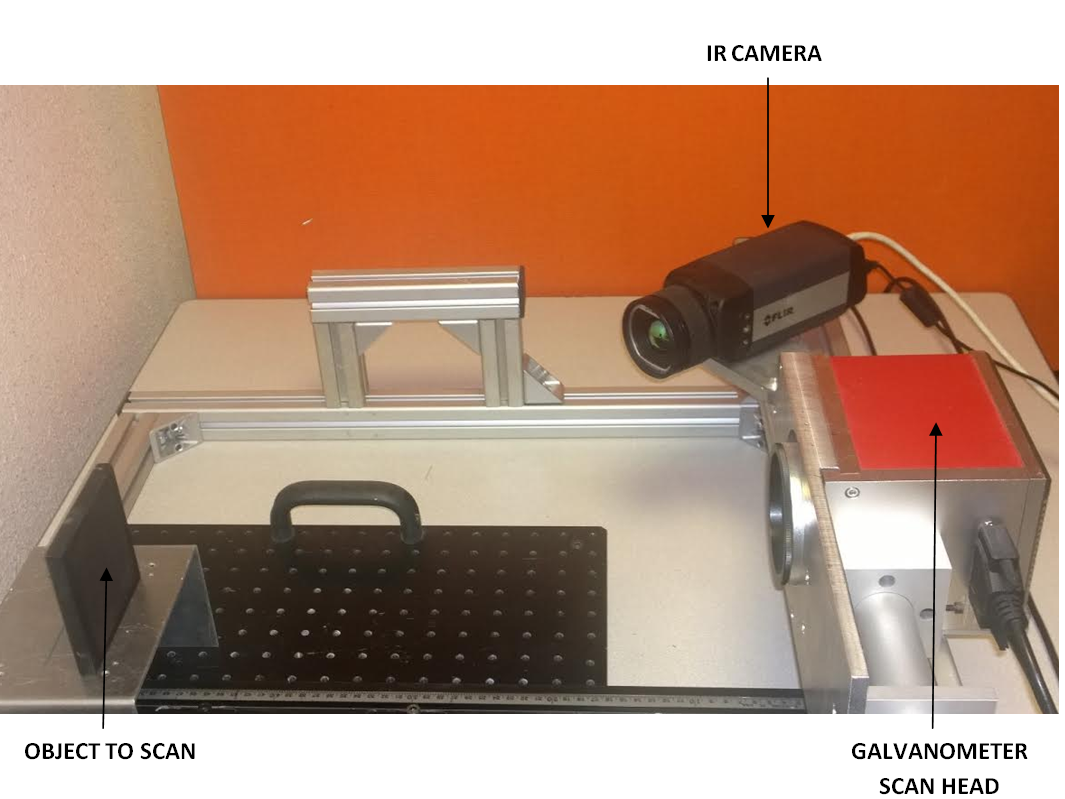
\includegraphics[width=0.3\linewidth]{fig4c.png}}
	%{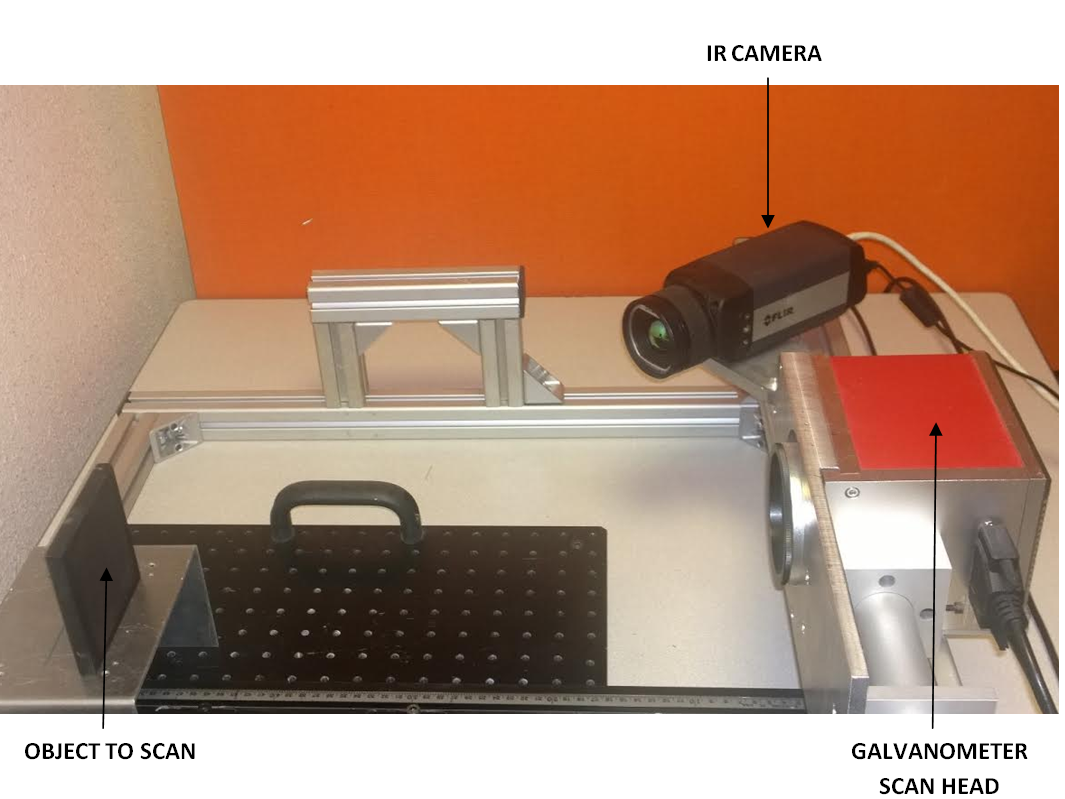
\includegraphics[width=0.7\linewidth]{fig4c.png}}
  %\hspace*{\fill}
  %\caption{%(a)-(b) Device for positioning the composite material - 
	%Scanner prototype.}
  %\label{fig:4}
%\end{figure}

Figure~\ref{fig:4} illustrates the complete scanning system setup. The system is composed by a FLIR~645 IR camera which captures the thermal radiation and an Nd~:YAG Laser system to stimulate the object surface. 
The FLIR~645 infrared camera provides a sensitivity range from \numrange{7.5}{14} \si{\micro \metre}.
The Nd~:YAG Laser system produces a step signal of \SI{1.5}{\second} period and the power of the laser beam is set up at \SI{1.5}{\watt}. 
A galvanometric mirror is used to control the position of the beam, which facilitates the object scanning with a \SI{1}{\milli \metre} resolution. 
During the experiment regarding the fiber orientation assessment, the motorized rotary stage ZABER T-RS60A is used.

\subsection{Experimental temperature profile}\label{subsec:42}

In order to validate the simulation results presented in Sect.\,\ref{subsec:311}, a set of thermal images are acquired. 
In these images, a defective area with a defect of \SI{0.5}{\milli \metre} below the surface and non-defective areas are excited with the laser beam (see Fig.\,\ref{fig:44}).
As previously predicted in the simulation section, the thermal response of a defective-area is different from the non-defective area, allowing non-through defects detection.

\subsection{Non-through defect detection}

%Figure~\ref{fig:5} reports two pairs of thermal images and their associated segmentation. The area of the segmented region in the image is more important when the laser impinges on a defective region of the object. By applying the segmentation method described in Sect.\,\ref{subsec:31}, we can detect the defective areas on the object's surface. 

Two type of material are used for the non-through defect detection: (i) steal plate and (ii) aluminum plate.
Both type of plates have non-through artificial defects, i.e. circle, square, triangle, and cross.
Defects are located between \SI{0.5}{\milli \metre} and \SI{2}{\milli \metre} below the observed surface for the aluminum plate and between \SI{1}{\milli \metre} and \SI{3}{\milli \metre} in the case of the steel plate.
The images are processed with the image processing algorithm presented in Sect.\,\ref{subsec:312}.
A 4-neighbors is considered during the region growing algorithm and a membership criterion of $0.2$, while the matrix $s_m$ is generated with $K=1.4$.
The results are depicted in Fig.\,\ref{fig:6} by superimposing with a color map on the raw image (i.e., red pixels are the non-through defects).

	%\graphicspath{ {./Figure/Figure7/} }
\begin{figure}
  \centering
	
  \hspace*{\fill}
  \subfigure[]{\label{subfig:44a}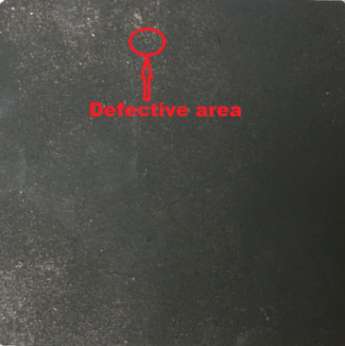
\includegraphics[width=0.3\linewidth]{fig3a.png}} \hfill
  \subfigure[]{\label{subfig:44b}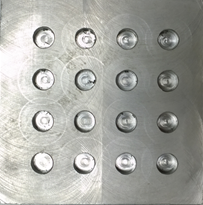
\includegraphics[width=0.3\linewidth]{fig3b.png}} 
  \hspace*{\fill} \\ \hspace*{\fill}
  \subfigure[]{\label{subfig:44c}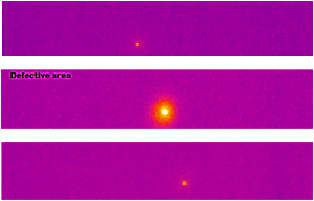
\includegraphics[width=0.3\linewidth]{fig3c.png}}
  %\subfigure[]{\label{subfig:3d}\includegraphics[width=0.3\linewidth]{fig3d.png}}
  \hspace*{\fill}
	
	  \caption{(a) Front side of the inspected material - (b) Back side of the inspected
		material - (c) Form of the thermal response of the material in the area with and without
		defect.}
		\label{fig:44}
		\end{figure}
  
	


%\begin{figure}
  %\centering
  %\hspace*{\fill}
  %\subfigure[]{\label{subfig:44a}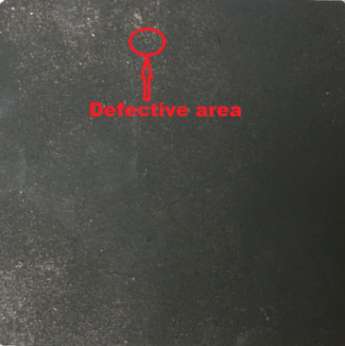
\includegraphics[width=0.3\linewidth]{fig3a.png}} \hfill
  %\subfigure[]{\label{subfig:44b}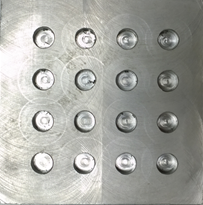
\includegraphics[width=0.3\linewidth]{fig3b.png}} 
  %\hspace*{\fill} \\ \hspace*{\fill}
  %\subfigure[]{\label{subfig:44c}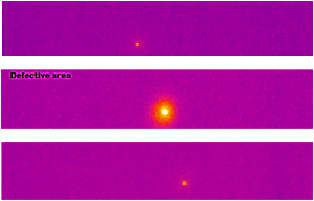
\includegraphics[width=0.3\linewidth]{fig3c.png}}
  %%\subfigure[]{\label{subfig:3d}\includegraphics[width=0.3\linewidth]{fig3d.png}}
  %\hspace*{\fill}
  %\caption{(a) Front side of the inspected material - (b) Back side of the inspected material 
	%- (c) Form of the thermal response of the material in the area with and without defect.}
  %\label{fig:44}
%\end{figure}

Figure~\ref{subfig:6a} shows a steel plate with circular non-through defects, in which defects have a diameter of 9, 7, 5, and \SI{3}{\milli \metre}, from left to right. 
Each defect is positioned at a different depth 1, 2, 2.5, and \SI{3}{\milli \metre}, from bottom to top. 
Only defects with depth less than or equal to \SI{2.5}{\milli \metre} are detected. 
However, the defects with a diameter less than \SI{5}{\milli \metre} are not detected as shown in Fig.\,\ref{subfig:6b}.
Besides, for the aluminum plate all defects are detected and the shape of the defect can be distinguished (see Fig.\,\ref{subfig:6d}). 

	%\graphicspath{ {./Figure/Figure8/}}
\begin{figure}
  \centering
	

  \hspace*{\fill}
  %\subfigure[]{\label{subfig:6a}\includegraphics[width=0.3\linewidth]{fig6a.png}} \hfill
  %\subfigure[]{\label{subfig:6b}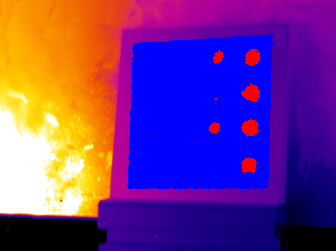
\includegraphics[width=0.3\linewidth]{fig6b.png}} 
  \subfigure[]{\label{subfig:6a}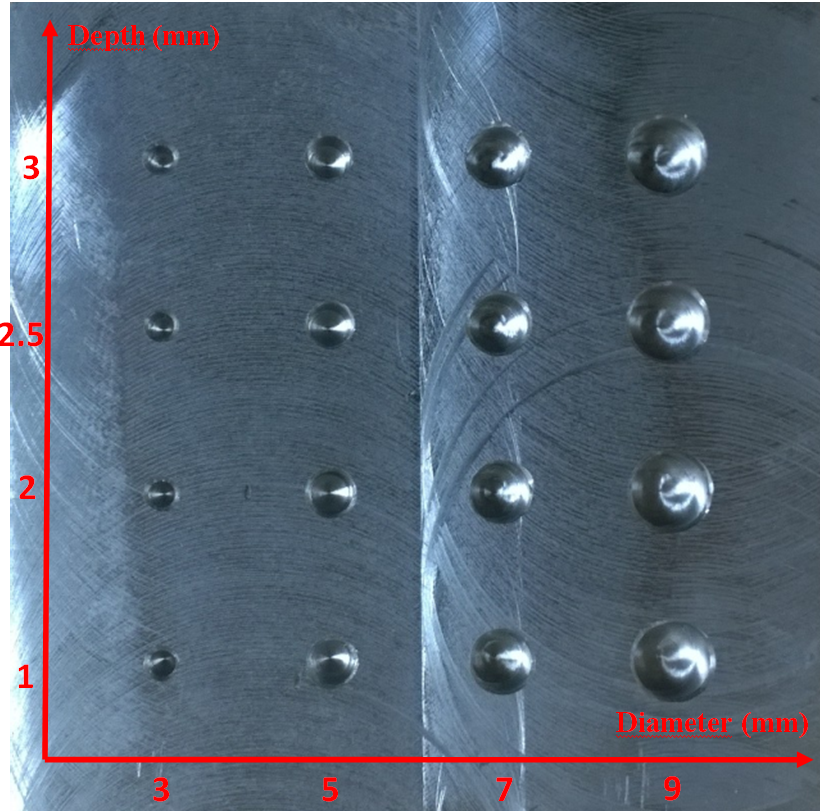
\includegraphics[width=0.3\linewidth]{fig7b.png}} \hfill
	\subfigure[]{\label{subfig:6b}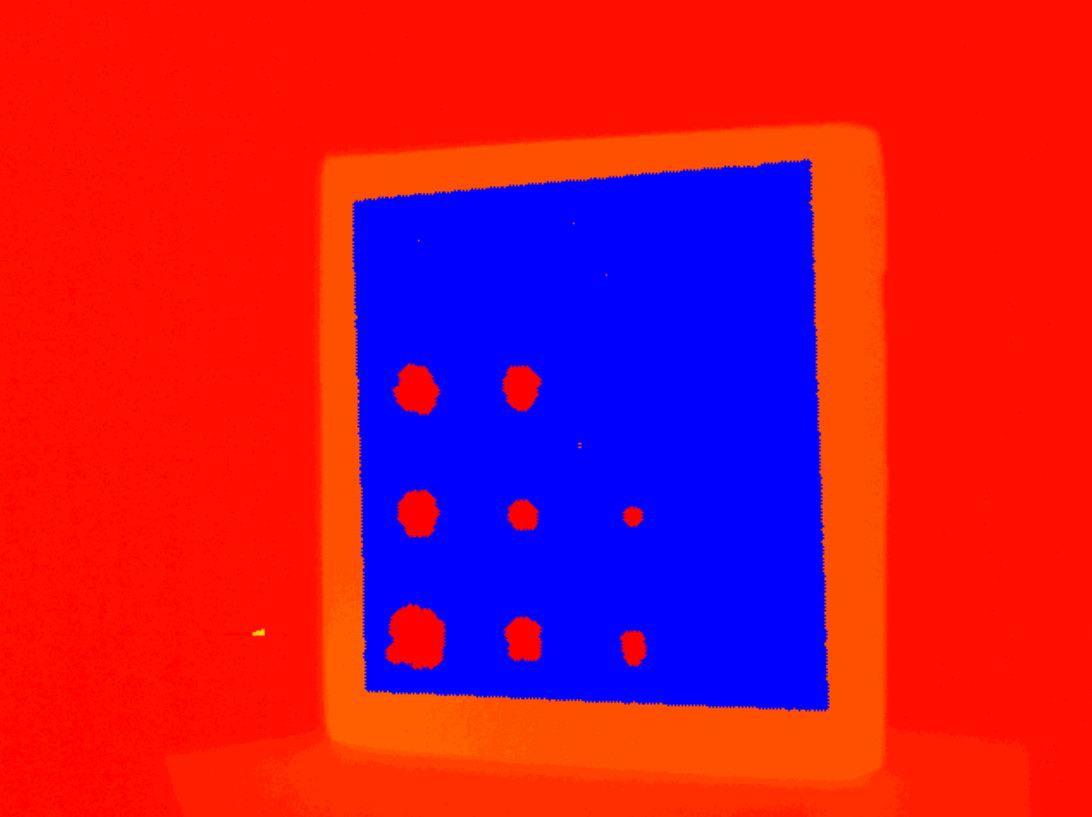
\includegraphics[width=0.3\linewidth]{fig7c.png}}
  \hspace*{\fill} \\ \hspace*{\fill}
  \subfigure[]{\label{subfig:6c}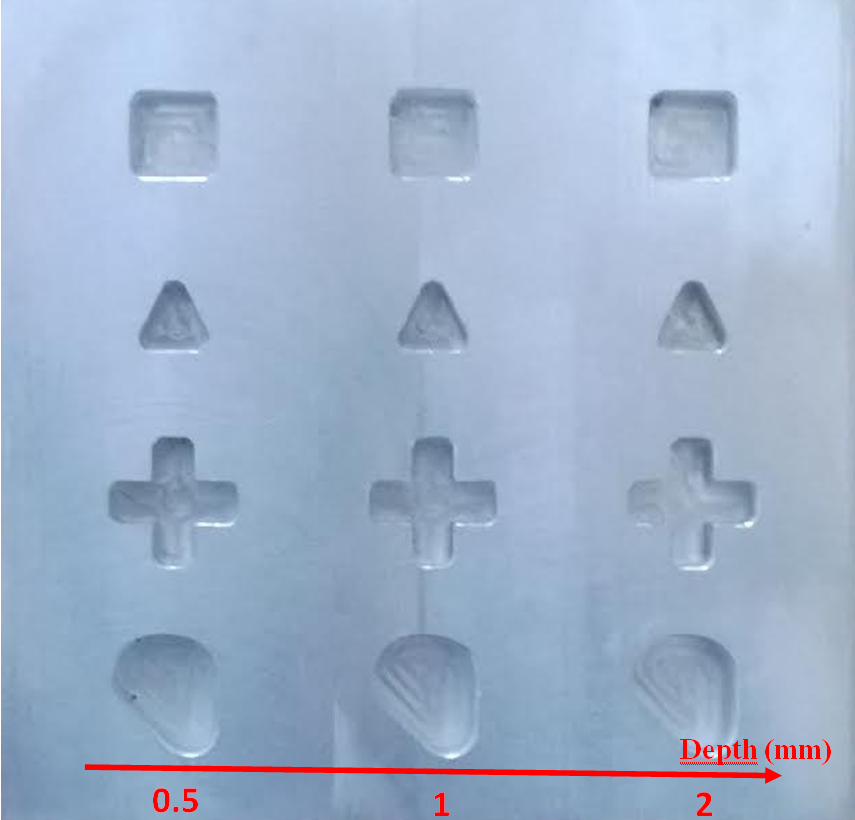
\includegraphics[width=0.3\linewidth]{fig6c.png}} \hfill
  \subfigure[]{\label{subfig:6d}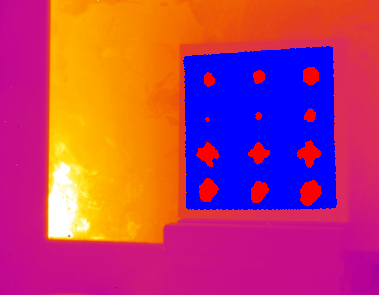
\includegraphics[width=0.3\linewidth]{fig6d.png}}
  \hspace*{\fill}
	
	  \caption{(a) and (c) Steel and aluminum objects - (b) and (d) Corresponding detection map.}
		\label{fig:6}
		\end{figure}
  
 
%\begin{figure}
  %\centering
  %\hspace*{\fill}
  %%\subfigure[]{\label{subfig:6a}\includegraphics[width=0.3\linewidth]{fig6a.png}} \hfill
  %%\subfigure[]{\label{subfig:6b}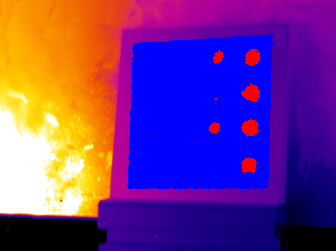
\includegraphics[width=0.3\linewidth]{fig6b.png}} 
  %\subfigure[]{\label{subfig:6a}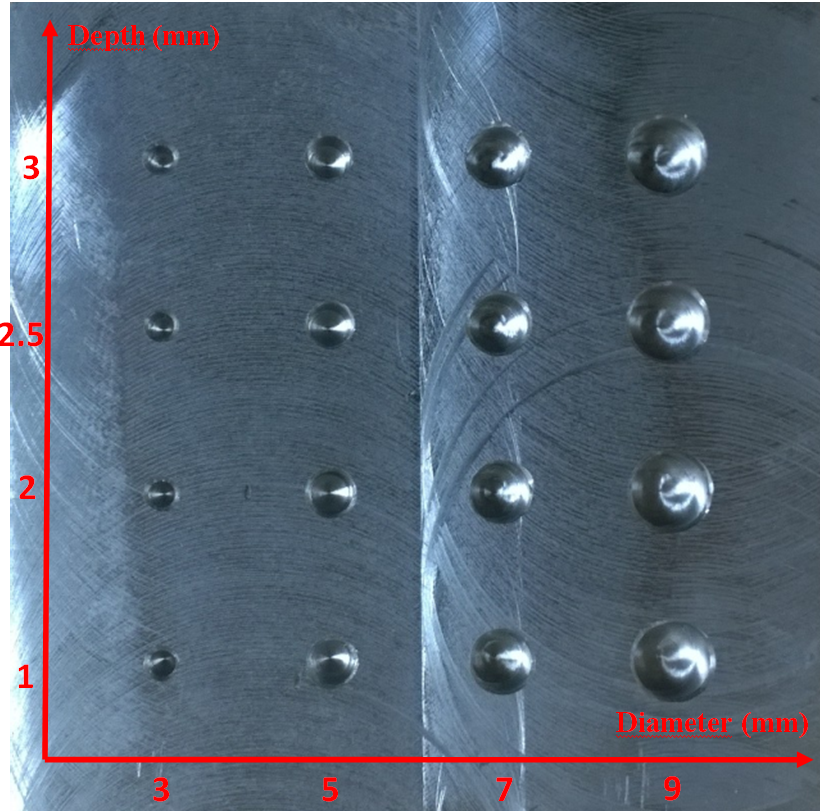
\includegraphics[width=0.3\linewidth]{fig7b.png}} \hfill
	%\subfigure[]{\label{subfig:6b}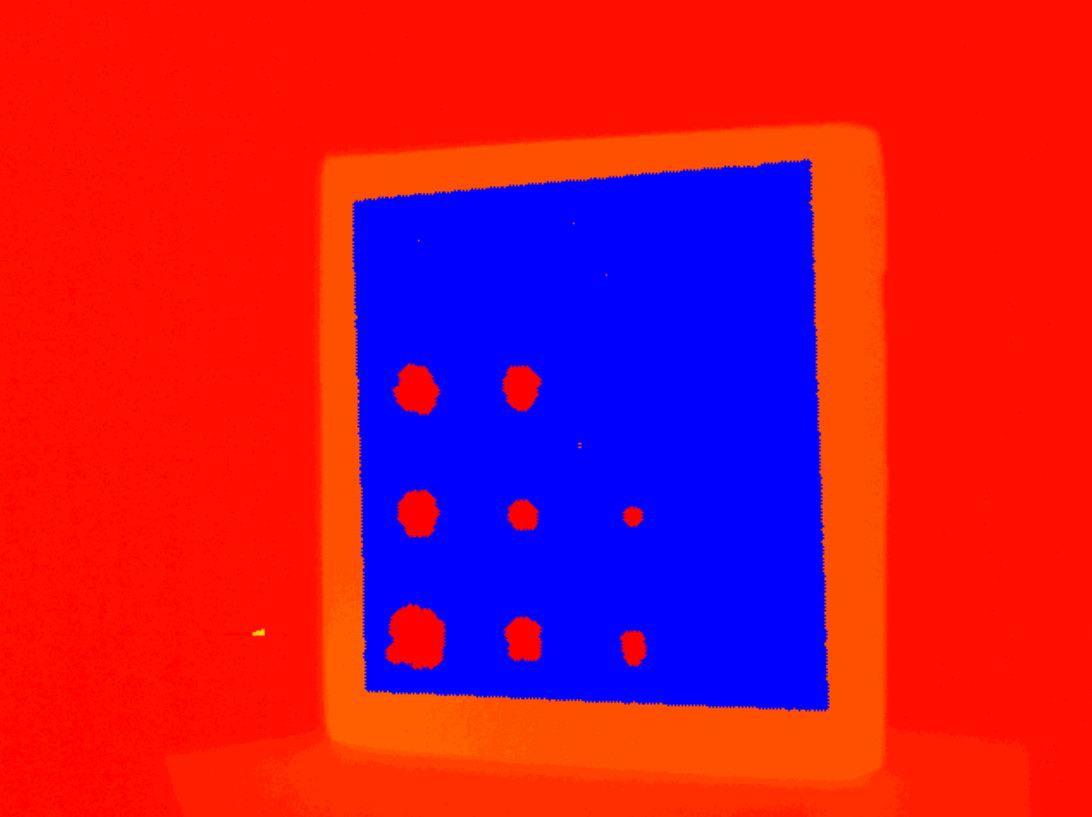
\includegraphics[width=0.3\linewidth]{fig7c.png}}
  %\hspace*{\fill} \\ \hspace*{\fill}
  %\subfigure[]{\label{subfig:6c}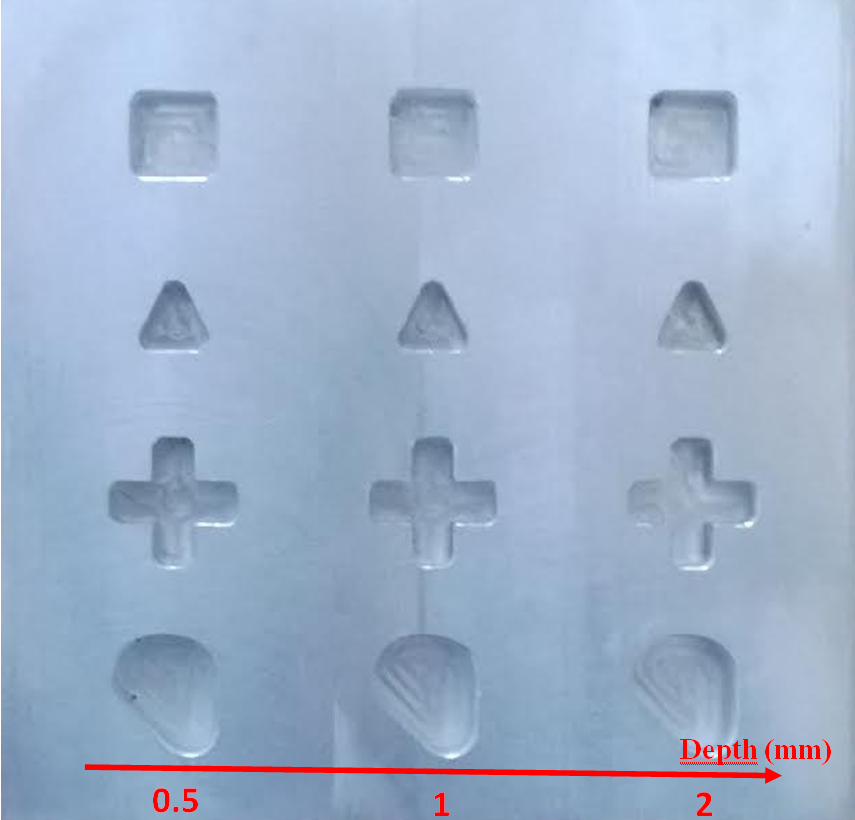
\includegraphics[width=0.3\linewidth]{fig6c.png}} \hfill
  %\subfigure[]{\label{subfig:6d}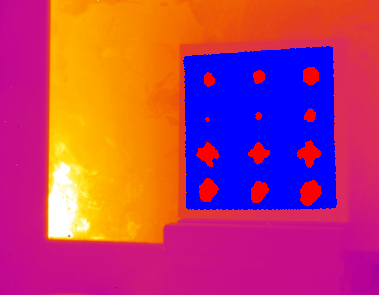
\includegraphics[width=0.3\linewidth]{fig6d.png}}
  %\hspace*{\fill}
  %\caption{(a) and (c) Steel and aluminum objects - (b) and (d) Corresponding detection map.}
  %\label{fig:6}
%\end{figure}

To study the repeatability of the technique, our framework is evaluated on steel plate with 16 identical circular defects located at \SI{1}{\milli \metre} depth and a \SI{10}{\milli \metre} diameter. 
The result of this experiment is depicted in Fig.\,\ref{subfig:7b}, in which all defects are successfully detected.


	%\graphicspath{ {./Figure/Figure9/}}
\begin{figure}
  \centering
	

  \hspace*{\fill}
  \subfigure[]{\label{subfig:7a}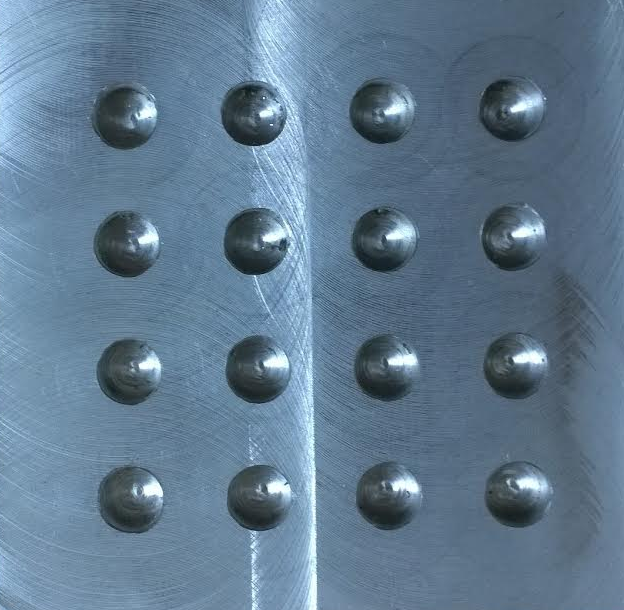
\includegraphics[width=0.3\linewidth]{fig7a.png}} \hfill
	\subfigure[]{\label{subfig:7b}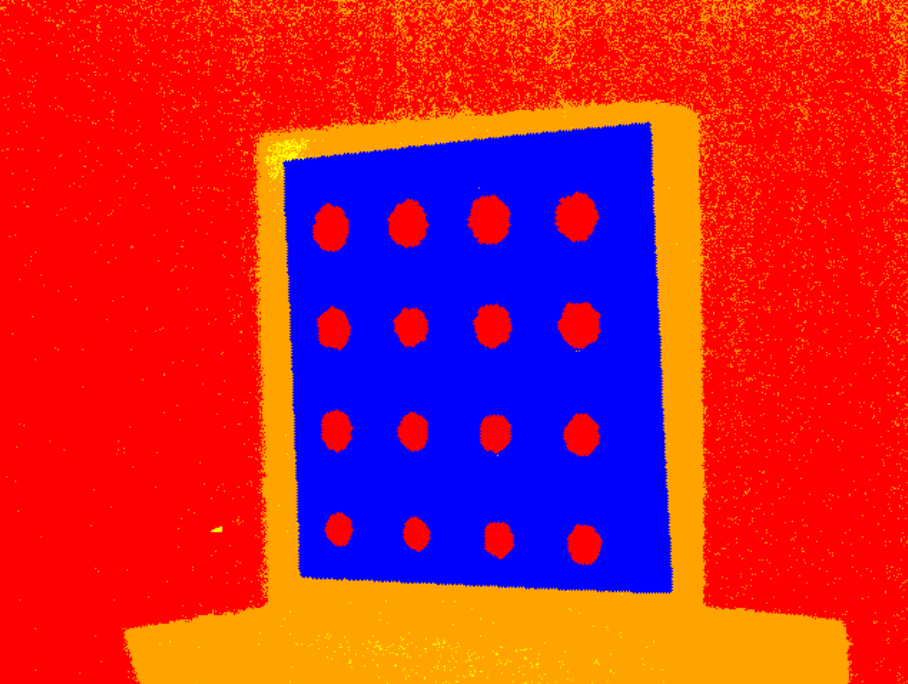
\includegraphics[width=0.3\linewidth]{fig7d.png}} 
  \hspace*{\fill}


	
		\caption{(a) Steel objects - (b) Corresponding detection map.}
  \label{fig:7}
\end{figure}
  

\subsection{Fusion of defect localization and 3D data}

To assess the quality of the fusion between the defect localization and the 3D data, a steel object is scanned (see Fig.\,\ref{subfig:8a}) to acquire a set of thermal images.
The steel object contains non-through circular defects in the planar part with a depth of \SI{1}{\milli \metre}.
The scanned area corresponds to the highlighted red delimitation depicted in Fig.\,\ref{subfig:8a}.
A similar method as proposed by Bajard~\emph{et al.}~\cite{Bajard2012} is used to obtain the 3D information and the defects are detected as in Sect.\ref{subsec:311}.
The coordinate system is the same for the 3D and defects information due to the fact that these data are acquired with the same system.
Therefore, the fusion between these data is straightforward, which overcome the matching problem faced by other methods as stated in the introduction section.

	%\graphicspath{ {./Figure/Figure10/}}
\begin{figure}
  \centering
	
  \hspace*{\fill}
  \subfigure[]{\label{subfig:8a}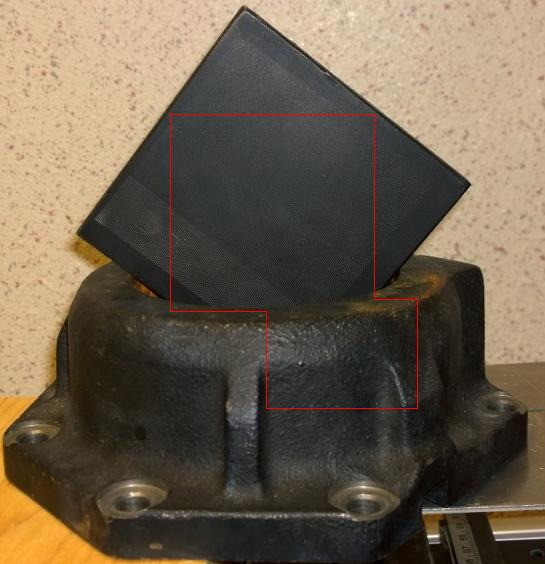
\includegraphics[width=0.3\linewidth]{fig8a.png}}\hfill
  \subfigure[]{\label{subfig:8b}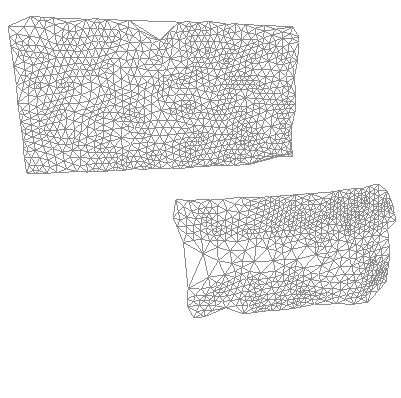
\includegraphics[width=0.3\linewidth]{fig8b.png}} 
	\hspace*{\fill} \\ \hspace*{\fill}
  \subfigure[]{\label{subfig:8c}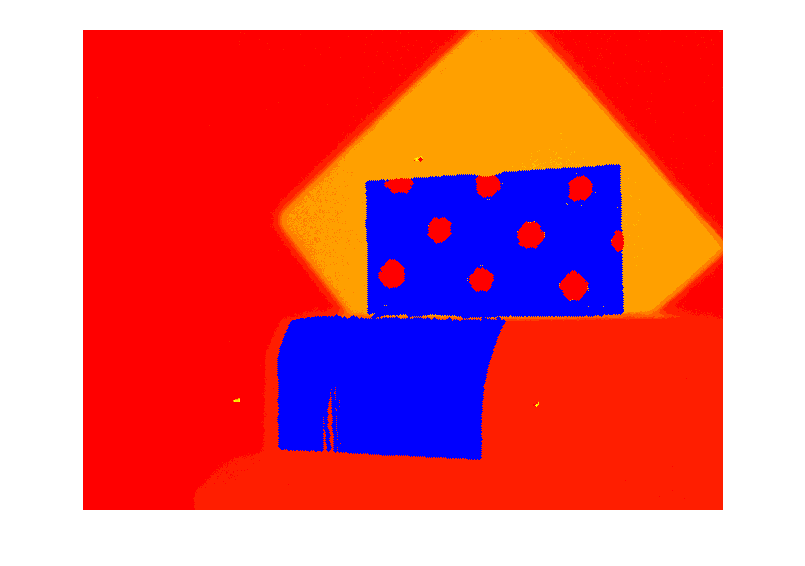
\includegraphics[width=0.3\linewidth]{fig8c.png}} \hfill
  \subfigure[]{\label{subfig:8d}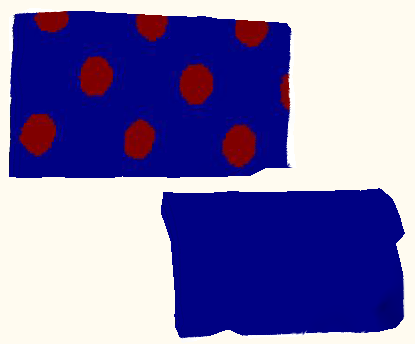
\includegraphics[width=0.3\linewidth]{fig8d.png}}
  \hspace*{\fill}
	
	\caption{(a) The specimen - (b) 3D mesh - (c) Corresponding detection map - (d) 3D mapping.}
  \label{fig:8}
\end{figure}
 

\subsection{Fiber orientations assessment}

In this section, we evaluate our framework at detecting the fiber orientation of carbon fiber composite material (see Fig.\,\ref{subfig:9a}).
The fiber orientation is estimated using the methodology presented in Sect.\,\ref{subsec:32}.
The initial experimental setup is as follows: 
firstly, the material is heated with the laser beam, the thermal radiation is recorded, and the orientation of the fiber is inferred. 
Secondly, the experiment is repeated by rotating the carbon plate at a \SI{90}{\degree} position.
The results of the ellipse fitting are depicted in Fig.\,\ref{subfig:9b}-\ref{subfig:9c}-\ref{subfig:9d}.
The algebraic fitting qualitatively shows an accurate fitting as shown in Fig.\,\ref{subfig:9d}, in which the blue dots represents the raw data, the green curve is the fitted ellipse, and the red line represents the ellipse major axis orientation.
As expected, the ellipse orientation follows the material rotation as depicted Fig.\,\ref{fig:10}.


	%\graphicspath{ {./Figure/Figure11/}}
\begin{figure}
  \centering
	

  \hspace*{\fill}
  \subfigure[]{\label{subfig:9a}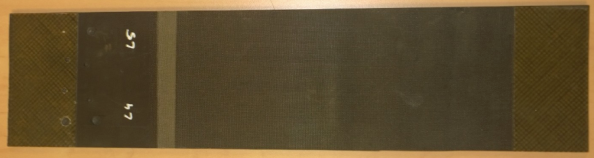
\includegraphics[width=0.3\linewidth]{fig9a.png}}
  \hspace*{\fill} \\ \hspace*{\fill}
  \subfigure[]{\label{subfig:9b}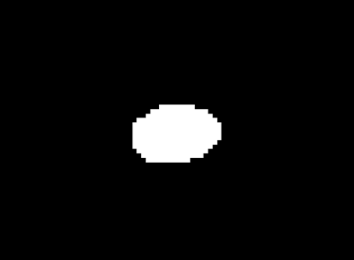
\includegraphics[width=0.3\linewidth]{fig9b.png}} \hfill
  \subfigure[]{\label{subfig:9c}
\includegraphics[width=0.3\linewidth]{fig9c.png}} \hfill
  \subfigure[]{\label{subfig:9d}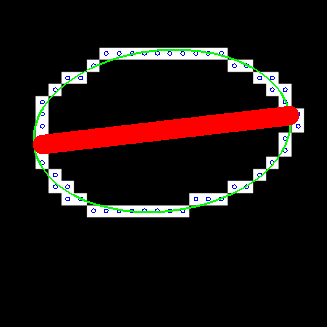
\includegraphics[width=0.3\linewidth]{fig9d.png}}
  \hspace*{\fill}
	  
		\caption{(a) The specimen - (b) Segmented thermal response - (c) Edge of the thermal
		response - (d) Ellipse fitting.}
		\label{fig:9}
		\end{figure}
  


	
	%\graphicspath{ {./Figure/Figure12/}}
\begin{figure}
  \centering

  \hspace*{\fill}
  \subfigure[]{\label{subfig:10a}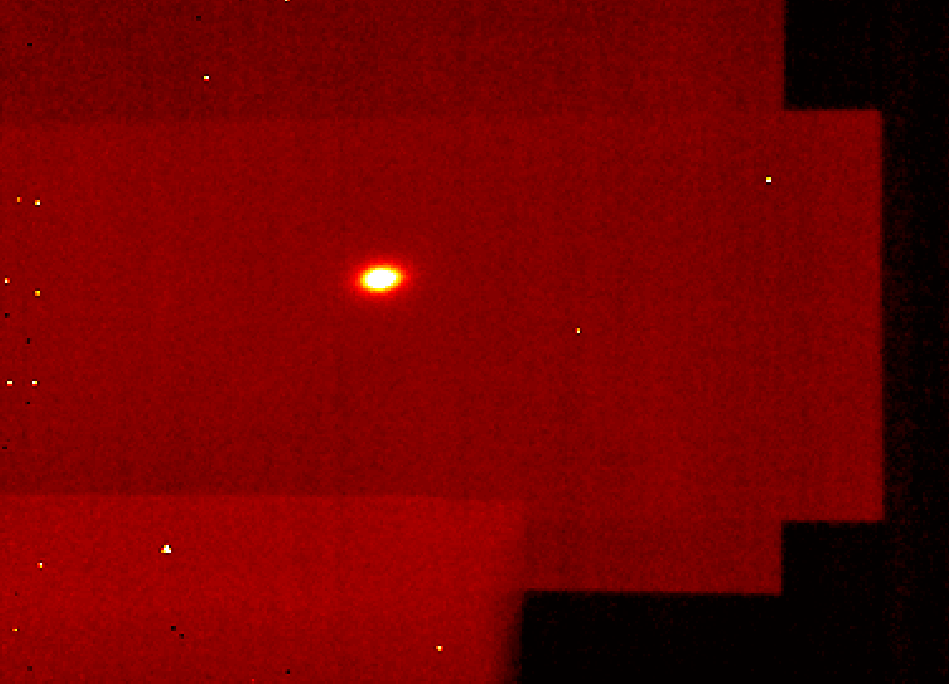
\includegraphics[width=0.3\linewidth]{fig10aa.png}} \hfill
  \subfigure[]{\label{subfig:10b}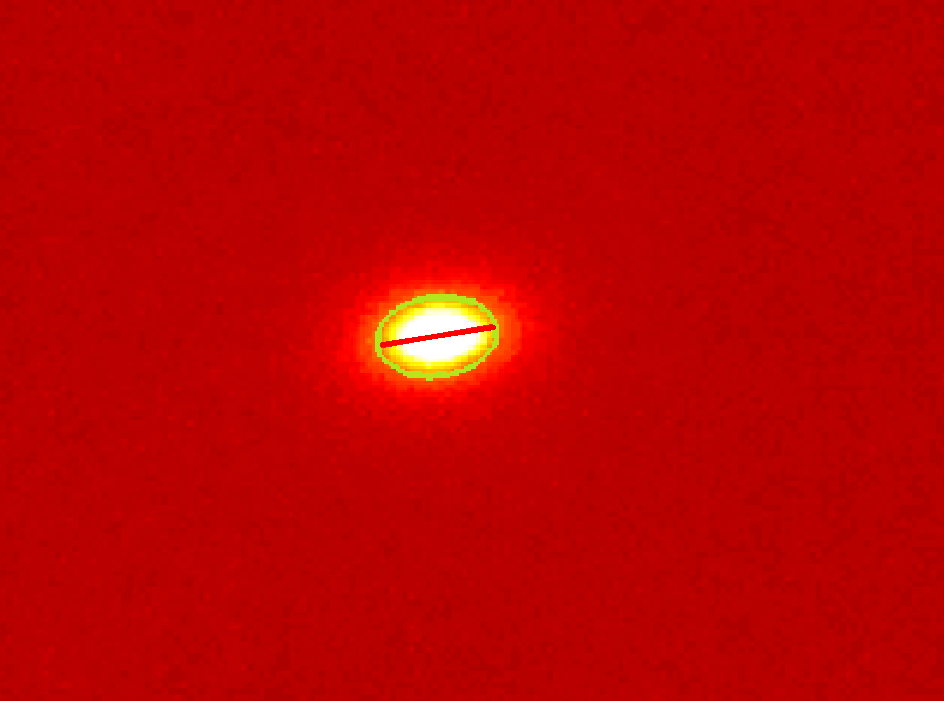
\includegraphics[width=0.3\linewidth]{fig10bb.png}} 
  \hspace*{\fill} \\ \hspace*{\fill}
  \subfigure[]{\label{subfig:10c}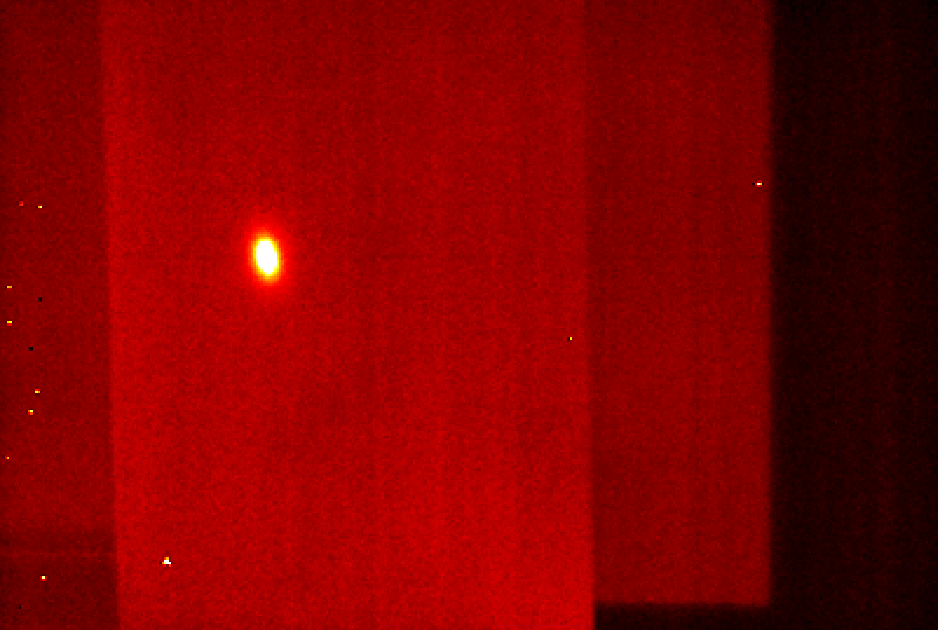
\includegraphics[width=0.3\linewidth]{fig10cc.png}} \hfill
  \subfigure[]{\label{subfig:10d}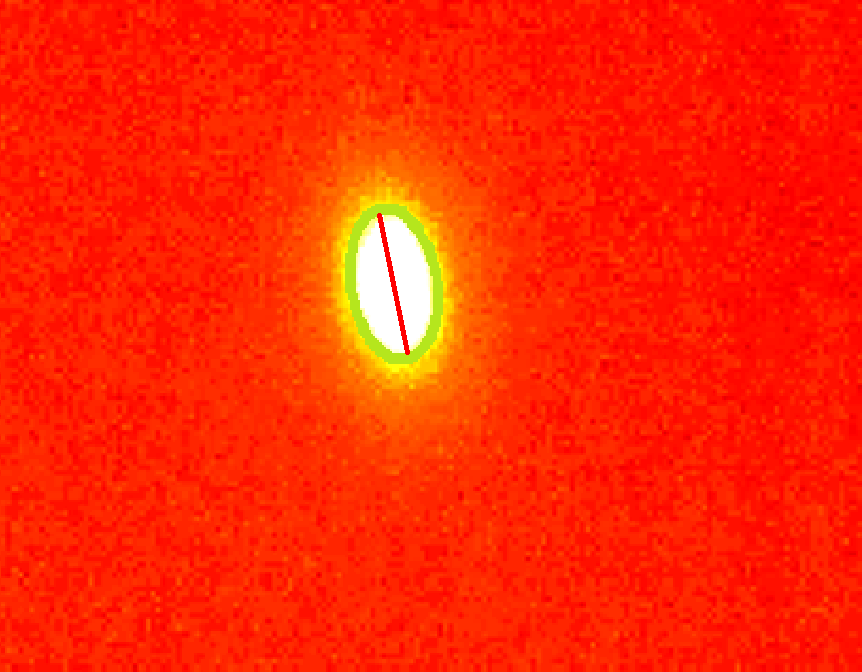
\includegraphics[width=0.3\linewidth]{fig10dd.png}}
  \hspace*{\fill}
	
	\caption{Example of fiber orientation detection: (a)-(b) horizontally oriented - (c)-(d)
		vertically oriented.}
		\label{fig:10}
		\end{figure}
  




The previous experiment are repeated acquiring 4 measurements for different orientations ranging from \SI{-10}{\degree} to \SI{-60}{\degree} with a step of \SI{10}{\degree}.
The absolute orientations are estimated and the mean and standard deviation are computed as presented in Table~\ref{tab:1}.
The average relative orientation is equal to \SI{10.8}{\degree} with a standard deviation of \SI{1.7}{\degree} and can be compared to the step which is set to \SI{10}{\degree}.

\begin{table}[h]
\caption{Fiber orientation evaluation.} 
\label{tab:1}
\begin{center}       
\begin{tabular}{lccccccc} 
\hline
\rule[-1ex]{0pt}{3.5ex}  & Initial position & \SI{-10}{\degree} & \SI{-20}{\degree} & \SI{-30}{\degree} & \SI{-40}{\degree} & \SI{-50}{\degree} & \SI{-60}{\degree} \\
\hline\hline
\rule[-1ex]{0pt}{3.5ex}  \multirow{4}{*}{Measurements} & 42.2 & 31.3 & 23.3 & 12.2 & 0.2 & -10.9 & -22.1  \\
\rule[-1ex]{0pt}{3.5ex}   & 42.8 & 31.1 & 22.5 & 13.9 & 0.4 & -10.9 & -21.7  \\
\rule[-1ex]{0pt}{3.5ex}   & 42.8 & 30.3 & 23.1 & 13.1 & -0.9 & -10.7 & -22.1  \\
\rule[-1ex]{0pt}{3.5ex}   & 43.7 & 31.8 & 22.9 & 13.1 & 0.4 & -10.9 & -22.1  \\
\hline
\rule[-1ex]{0pt}{3.5ex}  Average & 42.9 & 31.1 & 23.0 & 13.0 & 0.0 & -10.9 & -22.0 \\
\hline
\end{tabular}
\end{center}
\end{table}


